\newpage
\section{Concepts for Implementation}\label{sec:concepts}
In chapters above we discussed some possible security concepts and increments for the service location protocol. In following sections we will introduce our practical solutions to fulfill the requested requirements.\\
First of all we need to establish security groups, where users can communicate using encryption. To create those groups we combined the already implemented SLP scopes with a group key agreement protocol. For this purpose we took the Tree-based Group Diffie-Hellman protocol (TGDH). TGDH is a group key agreement protocol which we use to create and share security group keys (details about TGDH will be introduced in section \ref{sec:TGDH}). We will describe why we picked this protocol and how we integrated it into the SLP in detail.\\
Further we will discuss possible attacks on SLP which uses TGDH and the solutions we made to prevent them or provide reasons why we couldn't prevent them.

\subsection{Security Groups}
Like discussed above we propose to create security groups in an open network to establish security between some users and still offer all SLP functions there. To create a secured group within an open network we worked out a concept and a new workflow for our SecuredSLP. First of all a security group in SecuredSLP is a SLP scope in which the group members use encryption to communicate with each other, which means the group members all share a secret. To create and share a secret we used the TGDH protocol. There are some requirements to a security group which we should look at:
\begin{itemize}
  \item To join a secured group a user needs to know that there is such a group and this information should be announced as a plain text message, otherwise it isn't possible to get knowledge about such a group. The message should contain at least the information about the group name and where to get access to this group.
  \item After a user is allowed to join a group, he requires the shared secret of this group, the group key (see also sections \ref{sec:TGDH} and \ref{sec:keyexchange}). This key could be a manual distributed pre-shared key (e.g. an administrator provides network members with a group key) or a automatic generated and distributed key (e.g. a group agreement protocol which generates and distributes the group key)
  \item With a valid group key the user can decrypt all announced service information or offer services itself.
  \item If a user leaves a secured group, reasons could be for example an expired session key, the secured group key should be refreshed automatically.
\end{itemize}
We choose TGDH because it fulfills all the requirements above and we already found an implementation in java for it. But it is not necessary to use TGDH, so any other group key agreement protocol would work as well.\\
With TGDH each user within a secured group has several cryptographic keys.\\
\textbf{Group Shared Key (GSK):} This key is same for all group members and allows to access the secured group.\\
\textbf{Private-/Public-Key:} This is a key-pair that every user has and with those the users sign or verify the messages.

\subsection{Tree-based Group Diffie-Hellman (TGDH)}\label{sec:TGDH}
Tree-based Group Diffie-Hellman is a protocol-suite for group key management. It handles the key distribution between all network members. TGDH is based on a binary tree structure. But the tree structure is just logical and isn't connected with the real position of the network members. This protocol-suite handles several dynamic group events like a new member joins or leaves the group and two networks merge together or one network partitions in several networks. So TGDH implements four messages: \textsl{join}, \textsl{leave}, \textsl{merge} and \textsl{partition}\footnote{To secure SLP we only use the join and leave messages of the TGDH Protocol. For that reason the other messages won't be discussed in detail.}. But all of these messages have some common structures with following features:
\begin{itemize}
  \item Each network member computes the \textsl{group session key} out of the \textsl{group key} with a hash-function (the hash-function is the same for all members).
  \item Each \textsl{member session key} is just known to the member himself and shouldn't be published.
  \item In case a group gets larger, the \textsl{session keys} of new members will be included and some of old members have to refresh their \textsl{session key}.
  \item In case a group gets smaller, the \textsl{session keys} of the members, who left the group, will be deleted and at least one member of the group refreshes his \textsl{session key}.
  \item All protocol-messages are signed by the sender. For the digital signature TGDH uses RSA or DSA with SHA-1 hash-function. 
\end{itemize}
After any changes each member refreshes his \textsl{key-tree} independently from each other.\\

\subsubsection{Keys in TGDH}
There are several cryptographic keys which are used in TGDH.
\begin{description}
\item[Group key] $K_{<0,0>}$ which is represented as the root of the TGDH tree (compare with figure \ref{fig:tgdh_tree}).
\item[Group session key] $K_{\text{\textit{group}}}$ which is derived from the group key. $K_{\text{\textit{group}}} = h(K_{<0,0>})$, where $h()$ is a cryptographic hash-function.
\item[Member session key] $K_i$ is a session key for the member $M_i$. 
\item[Blinded key] $BK_i$ is a key which can be calculated from the member session key $K_i$ with the function $BK_i = f(K_i)$, where $f() = g^k~mod~p$ with $g$ as generator and $p$ as a prime.
\end{description}
Furthermore there are also key sets a member has knowledge about. Each member knows all keys and their corresponding blinded keys in his path from the leaf to the root in the tree. For example member $M_2$ in the figure \ref{fig:tgdh_tree} knows the set of keys $\{K_{<2,1>}, K_{<1,0>}, K_{<0,0>}\}$ and the set of blinded keys $\{BK_{<2,1>}, BK_{<1,0>}, BK_{<0,0>}\}$. With that information it is possible to compute any other key:
\begin{align*}
K_{<l,v>} &= (BK_{<l+1, 2v+1>})^{K_{<l+1, 2v>}}~mod~p\\
&= (BK_{<l+1, 2v>})^{K_{<l+1, 2v+1>}}~mod~p\\
&= g^{K_{<l+1, 2v>}K_{<l+1, 2v+1>}}~mod~p\\
&= f(K_{<l+1, 2v>}K_{<l+1, 2v+1>})
\end{align*}
It is also possible to compute the group key out of that information. For member $M_2$ the calculation would be:
\begin{align*}
K_{<0,0>} &= (BK_{<1,1>})^{K_{<1,0>}}~mod~p\\
&= (BK_{<1,1>})^{(BK_{<2,1>})^{K_{<2,0>}}}~mod~p
\end{align*}
\begin{figure}[!h]
\centering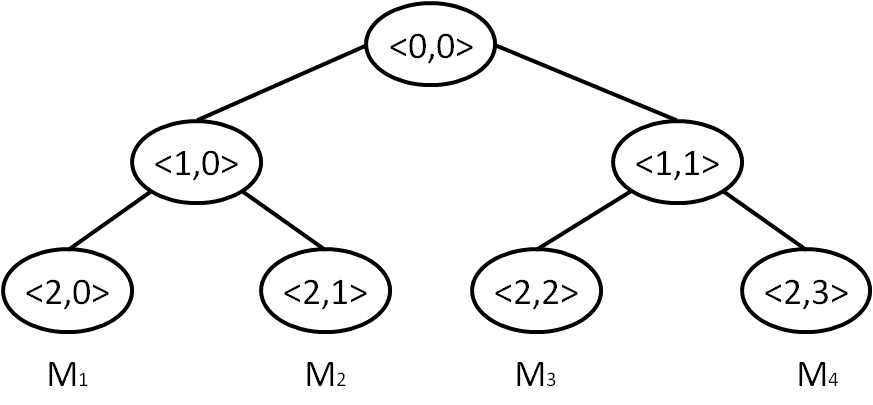
\includegraphics[width=0.5\textwidth]{Images/tgdh_tree}
\caption{Example of a tree structure in TGDH}
\label{fig:tgdh_tree}
\end{figure}

\subsubsection{Join protocol}
Assume a group with three members $\{M_1, M_2, M_3\}$ and a new member $M_4$ who wants to join this group. $M_4$ initialize the join protocol by sending a \textit{JoinMessage} to the group via multicast. The message contains the blinded key of $M_4$. First of all the join position for $M_4$ is calculated and a \textit{sponsor} is chose. The sponsor is the member whose leaf is placed on the insert position of the new member. In this case all members insert a new joint and a new leaf in their tree and delete all blinded keys in the path of the sponsor. Additionally the sponsor generates the new group session key and all keys and blinded keys in his path. Finally the sponsor sends the new tree $\widehat{T}$ and a set of all blinded keys via a multicast message. Member $M_1$ and $M_2$ can just calculate the group key after they received the new tree $\widehat{T}$. The tree update is shown in figure \ref{fig:tgdh_join}.
\begin{figure}[!h]
\centering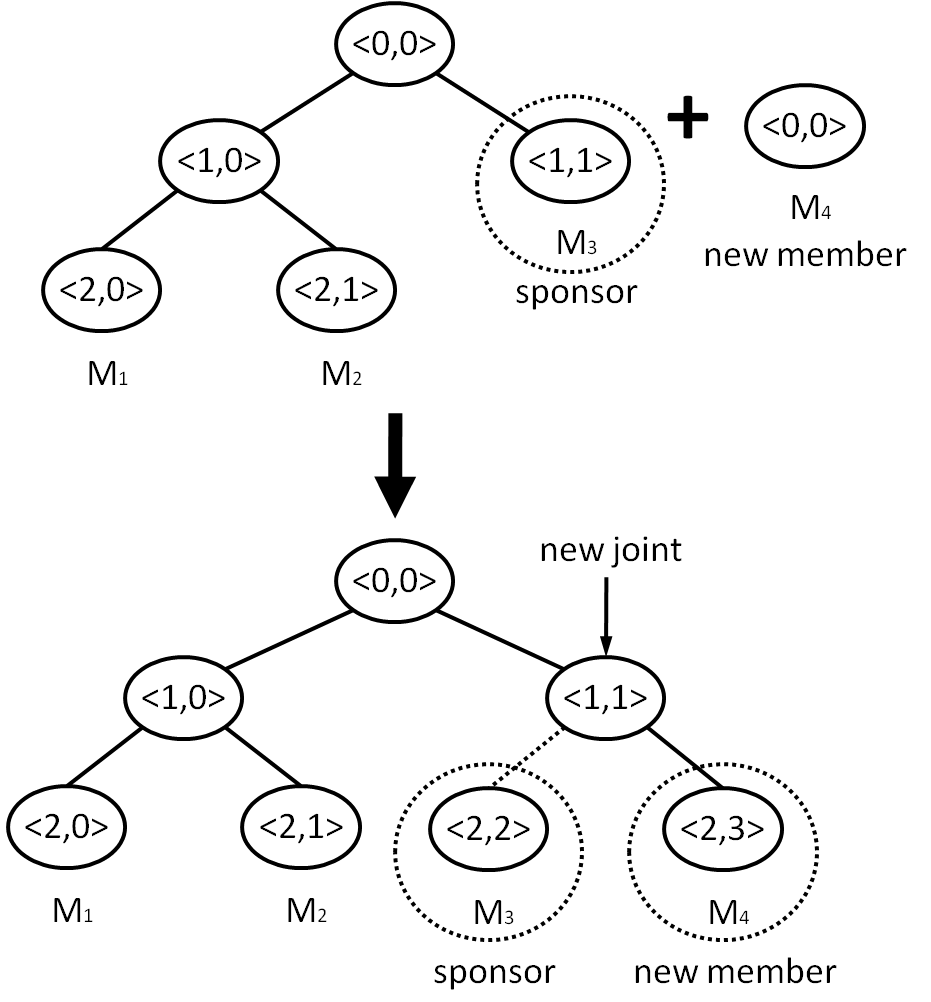
\includegraphics[width=0.5\textwidth]{Images/tgdh_join}
\caption{Tree update after a join of a new member}
\label{fig:tgdh_join}
\end{figure}

\subsubsection{Leave protocol}
To leave the group a member sends a \textit{LeaveMessage} via multicast to the group. Same as in join protocol, a sponsor is chose. All members remove the leaf and his father joint from the tree. Also they remove all keys and blinded keys in the corresponding path. Additionally the sponsor generates new session key and computes all keys and blinded keys in his path. In the end sponsor sends the new tree $\widehat{T}$ and a set of all blinded keys via broadcast to the group. After receiving the new tree, all other members are able to compute the new group key. The corresponding tree update is illustrated in figure \ref{fig:tgdh_leave}.
\begin{figure}[!h]
\centering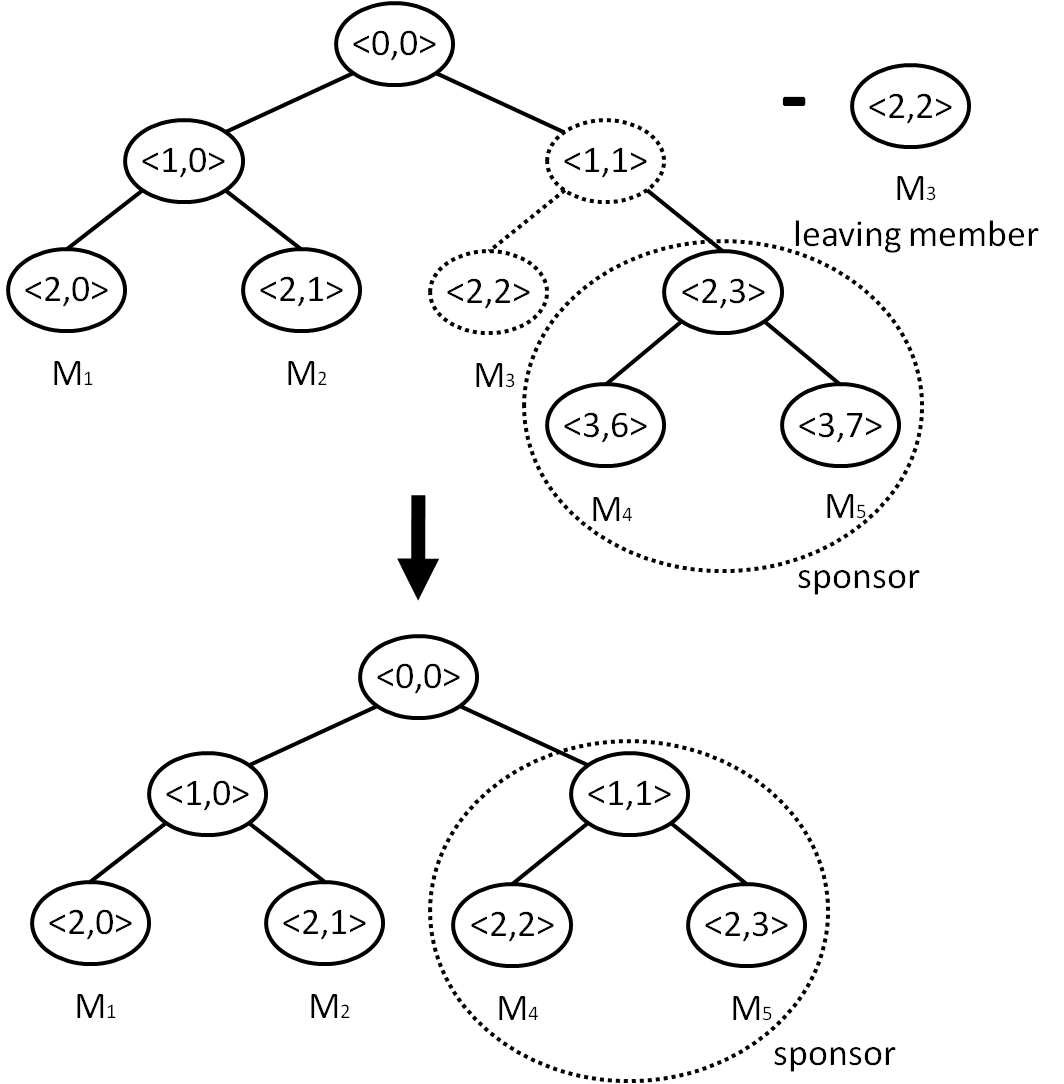
\includegraphics[width=0.5\textwidth]{Images/tgdh_leave}
\caption{Tree update after a member left the group}
\label{fig:tgdh_leave}
\end{figure}